% !TEX program = xelatex
\documentclass[aspectratio=169,8pt]{beamer}

% metroplis theme
\usetheme[numbering=counter,progressbar=none]{metropolis}

\usefonttheme{default} 
\usepackage[sfdefault,book,medium]{FiraSans}
\usepackage{FiraMono}

\usepackage{tikz}
\usetikzlibrary{arrows.meta,positioning,calc,fit}
\usepackage{amsmath}
\usepackage{booktabs}
\usepackage{xcolor}
\usepackage{pgfpages}

\usepackage[many]{tcolorbox} 

\setbeameroption{hide notes}

% Color Palette
\definecolor{mDarkTeal}{HTML}{03383b}  % Header bg, Title text, Blue box border
\definecolor{mLightGray}{HTML}{FAFAFA} % Main slide background
\definecolor{tealBorder}{HTML}{6A9A9D} % Teal box border
\definecolor{tealBg}{HTML}{F2F6F6}     % Teal box body background
\definecolor{blueBg}{HTML}{EBECEE}     % Blue box body background
\definecolor{mText}{HTML}{041f25}      % Default text color
\definecolor{mRed}{HTML}{f97171}       

\setbeamercolor{normal text}{fg=mText,bg=mLightGray}
\setbeamercolor{frametitle}{fg=white,bg=mDarkTeal}
\setbeamercolor{title separator}{fg=mDarkTeal}
\setbeamercolor{itemize item}{fg=mDarkTeal}
\setbeamercolor{itemize subitem}{fg=mDarkTeal}
\setbeamercolor{alerted text}{fg=mRed}

\setbeamertemplate{itemize item}{\textbullet}
\setbeamertemplate{itemize subitem}{$\circ$}

\setbeamerfont{frametitle}{size=\large,series=\normalfont} 
\setbeamerfont{title}{size=\LARGE,series=\normalfont}
\setbeamerfont{subtitle}{size=\large,series=\normalfont}
\setbeamerfont{author}{size=\normalsize}

% ---------- Custom Info Boxes (matching screenshots exactly) ----------
\newtcolorbox{tealbox}[1]{
  colback=tealBg,
  colframe=tealBorder,
  coltitle=white,
  title={#1},
  arc=3pt,
  boxrule=1.5pt,
  left=6pt, right=6pt, top=4pt, bottom=4pt,
  fonttitle=\normalsize,
  fontupper=\small,
  boxsep=2pt
}

\newtcolorbox{bluebox}[1]{
  colback=blueBg,
  colframe=mDarkTeal,
  coltitle=white,
  title={#1},
  arc=3pt,
  boxrule=1.5pt,
  left=6pt, right=6pt, top=4pt, bottom=4pt,
  fonttitle=\normalsize,
  fontupper=\small,
  boxsep=2pt
}

% TikZ styles
\tikzset{
  arr/.style={-{Latex[length=2.2mm]}, thick, mDarkTeal!75},
  redarr/.style={-{Latex[length=2.2mm]}, thick, red!75},
  bigarr/.style={-{Latex[length=3mm]}, very thick, mDarkTeal!80},
  gpu/.style={font=\normalsize\bfseries, text=mDarkTeal},
  shard/.style={draw=#1!80!black, fill=#1!13, rounded corners=2pt, thick,
    minimum width=0.80cm, minimum height=0.45cm, font=\scriptsize,
    text=#1!60!black, align=center},
  stage/.style={draw=#1!80!black, fill=#1!11, rounded corners=5pt, thick,
    minimum width=2.55cm, minimum height=0.72cm, align=center,
    font=\footnotesize, text=mDarkTeal},
  callout/.style={draw=mDarkTeal!18, fill=blueBg!80, rounded corners=5pt,
    text width=5.2cm, align=left, inner sep=6pt, font=\footnotesize},
  mini/.style={draw=mDarkTeal!18, fill=blueBg!75, rounded corners=4pt,
    text width=4.55cm, align=left, inner sep=5pt, font=\scriptsize},
  take/.style={draw=mDarkTeal!80!black, fill=tealBg, rounded corners=7pt, thick,
    text width=13.4cm, minimum height=0.54cm, align=center,
    inner sep=3.5pt, font=\small, text=mDarkTeal}
}
\newcommand{\takeaway}[1]{\begin{center}\begin{tikzpicture}\node[take]{#1};\end{tikzpicture}\end{center}}

% ---------- Title Page Info ----------
\title{Full Sharded Data Parallel}
\subtitle{Lorem Ipsum}
\author{Utshav Saha\\[0.5cm]\footnotesize sahaushno@gmal.com}
\date{} % Empty date to match the reference image

\begin{document}

% ================================================================
% Title Frame
\begin{frame}[plain] % 'plain' removes header/footer for the title page
  \maketitle
\end{frame}

% ================================================================
\begin{frame}[t]{11. Sharding: split one big thing into pieces}
\transfade[duration=0.2]
\begin{columns}[T,onlytextwidth]
\column{0.50\textwidth}
\vspace{0.15cm}
\begin{tikzpicture}[x=1cm,y=1cm]
  \node[font=\normalsize\bfseries] at (0,2.8) {One large model state};
  \draw[rounded corners=9pt, draw=mDarkTeal, fill=tealBg, very thick] (-2.0,1.75) rectangle (2.0,2.35);
  \node[font=\large\bfseries,text=mDarkTeal] at (0,2.05) {MODEL STATE};
  \only<2->{
    \draw[bigarr] (0,1.55) -- (0,0.92);
    \node[font=\normalsize\bfseries] at (0,0.65) {Break it into shards};
    \foreach \x/\c/\s in {-1.5/red/$S_0$,-0.5/green/$S_1$,0.5/blue/$S_2$,1.5/orange/$S_3$}{
      \node[shard=\c, minimum width=0.84cm,minimum height=0.52cm] at (\x,-0.15) {\s};
    }
  }
  \only<3->{
    \foreach \x/\g in {-1.5/GPU 0,-0.5/GPU 1,0.5/GPU 2,1.5/GPU 3}{
      \draw[arr] (\x,-0.48) -- (\x,-0.90);
      \node[gpu,font=\footnotesize\bfseries] at (\x,-1.18) {\g};
    }
  }
\end{tikzpicture}

\column{0.47\textwidth}
\vspace{0.2cm}
\begin{bluebox}{Story intuition}
In games, shards are small pieces that together complete one item. FSDP uses the same idea for training state.
\end{bluebox}
\vspace{0.12cm}
\begin{itemize}
  \item<2-> Split one large state into pieces.
  \item<3-> Give different pieces to different GPUs.
  \item<4-> Reconstruct a full piece of the model only when computation needs it.
\end{itemize}
\end{columns}
\vspace{1.5 cm}
\only<4->{\takeaway{FSDP starts by \textbf{splitting} model state instead of \textbf{replicating} it.}}
\end{frame}

% ================================================================
\begin{frame}[t]{12. What exactly is sharded?}
\transfade[duration=0.2]
\begin{columns}[T,onlytextwidth]
\column{0.5\textwidth}
\vspace{0.15cm}
\begin{center}
  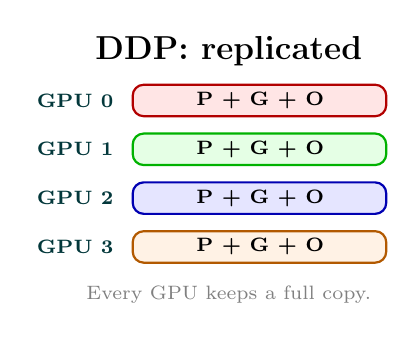
\begin{tikzpicture}[x=1cm,y=1cm]
  \node[font=\bfseries\large] at (0,2.8) {DDP: replicated};
  \foreach \i/\y/\c in {0/2.18/red,1/1.56/green,2/0.94/blue,3/0.32/orange}{
    \node[gpu,font=\scriptsize\bfseries] at (-1.95,\y) {GPU \i};
    \draw[rounded corners=4pt,draw=\c!70!black,fill=\c!10,thick] (-1.22,\y-0.20) rectangle (2.00,\y+0.20);
    \node[font=\scriptsize\bfseries] at (0.40,\y) {P + G + O};
  }
  \node[font=\scriptsize,text=gray,align=center] at (0,-0.28) {Every GPU keeps a full copy.};
\end{tikzpicture}
\end{center}


\column{0.5\textwidth}
\vspace{0.15cm}
\begin{center}
  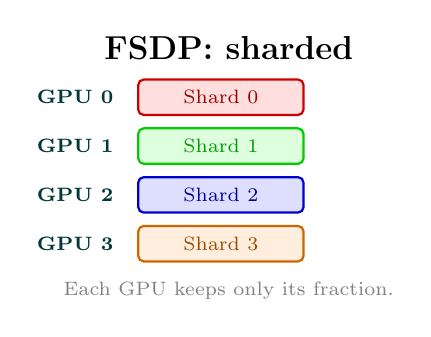
\begin{tikzpicture}[x=1cm,y=1cm]
  \node[font=\bfseries\large] at (0,2.8) {FSDP: sharded};
  \only<2->{
  \foreach \i/\y/\c/\s in {0/2.18/red/Shard 0,1/1.56/green/Shard 1,2/0.94/blue/Shard 2,3/0.32/orange/Shard 3}{
    \node[gpu,font=\scriptsize\bfseries] at (-1.95,\y) {GPU \i};
    \node[shard=\c, minimum width=2.1cm] at (-0.10,\y) {\s};
  }
  \node[font=\scriptsize,text=gray,align=center] at (0,-0.28) {Each GPU keeps only its fraction.};
  }
\end{tikzpicture}
\end{center}

\end{columns}
\vspace{0.08cm}
\only<3->{
\begin{center}
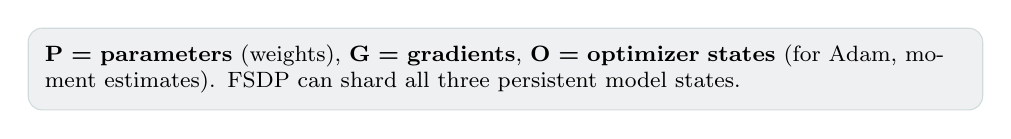
\begin{tikzpicture}
  \node[callout,text width=11.7cm] {\textbf{P = parameters} (weights), \textbf{G = gradients}, \textbf{O = optimizer states} (for Adam, moment estimates). FSDP can shard all three persistent model states.};
\end{tikzpicture}
\end{center}}
\vspace{-0.06cm}
\only<4->{\takeaway{Idealized persistent model-state memory per GPU scales roughly as $\frac{P+G+O}{N}$.}}
\end{frame}

% ================================================================
\begin{frame}[t]{13. The first problem: a layer cannot compute from one shard}
\transfade[duration=0.2]
\begin{columns}[T,onlytextwidth]
\column{0.50\textwidth}
\vspace{0.18cm}
\begin{tikzpicture}[x=1cm,y=1cm]
  \node[gpu] at (-1.25,2.35) {GPU 0 owns only};
  \node[shard=mRed!80!black,fill=mRed!10,minimum width=1.1cm,minimum height=0.60cm] (w0) at (0.60,2.35) {$W_0$};
  \node[font=\scriptsize,text=gray] at (-0.9,1.75) {one piece of a layer's weight tensor};
  \only<2->{
    \node[draw=mRed!80!black,fill=mRed!10,rounded corners=7pt,very thick,minimum width=3.5cm,minimum height=0.95cm,align=center] (calc) at (0,0.78) {Layer operation\\[-1mm] $y=Wx$};
    \draw[redarr] (w0.south) to[out=-60, in=60] (calc.north east);
    \node[font=\Huge\bfseries,text=mRed] at (2.35,0.78) {?};
  }
  \only<3->{\node[font=\footnotesize,align=center] at (0,-0.15) {$W$ means the \textbf{complete} tensor,\\not only $W_0$.};}
\end{tikzpicture}

\column{0.47\textwidth}
\vspace{0.25cm}
\only<2->{\begin{tealbox}{The tension}
Sharding saves memory, but the current layer normally needs its full parameter tensor to run the matrix operations.
\end{tealbox}}
\vspace{0.15cm}
\only<3->{
\begin{center}
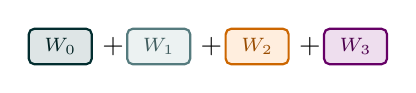
\begin{tikzpicture}
  \node[shard=mDarkTeal] at (0,0) {$W_0$};
  \node at (0.67,0) {$+$};
  \node[shard=tealBorder] at (1.25,0) {$W_1$};
  \node at (1.92,0) {$+$};
  \node[shard=orange] at (2.50,0) {$W_2$};
  \node at (3.17,0) {$+$};
  \node[shard=violet] at (3.75,0) {$W_3$};
\end{tikzpicture}
\end{center}}
\end{columns}
\vspace{0.08cm}
\only<4->{\takeaway{So FSDP must \textbf{temporarily collect} the missing parameter shards before computation.}}
\end{frame}

% ================================================================
\begin{frame}[t]{14. All-Gather: temporarily rebuild the current FSDP unit}
\transfade[duration=0.2]

\begin{center}
\begin{tikzpicture}[x=1cm,y=1cm,
    rank/.style={draw=mDarkTeal!28, fill=blueBg!55, rounded corners=4pt},
    ranklab/.style={font=\scriptsize\bfseries, text=mDarkTeal},
    note/.style={font=\tiny, text=mDarkTeal!55},
    capt/.style={font=\footnotesize, text=mDarkTeal, align=center},
    flow/.style={-{Latex[length=2.1mm,width=1.7mm]}, semithick},
    bandtag/.style={font=\scriptsize\itshape, text=orange!45!black}]

  \path (-6.80,-1.80) rectangle (6.80,3.76);

  \node[capt] at (0,3.42)
    {\textbf{(a) Before.}~Each rank persists one disjoint shard $W_i$ of this unit's parameter tensor.};

  \foreach \i/\x/\c/\s in {0/-5.40/mDarkTeal/$W_0$,1/-1.80/tealBorder/$W_1$,2/1.80/orange/$W_2$,3/5.40/violet/$W_3$}{
    \draw[rank] (\x-1.40,1.65) rectangle (\x+1.40,3.00);
    \node[ranklab] at (\x,2.75) {GPU \i};
    \node[shard=\c,minimum width=1.00cm,minimum height=0.44cm] at (\x,2.26) {\s};
    \node[note] at (\x,1.85) {persistent: $|W|/N$};
  }

  \only<2->{
    \foreach \x/\c in {-5.40/mDarkTeal,-1.80/tealBorder,1.80/orange,5.40/violet}{
      \draw[flow,draw=\c!75!black] (\x,1.65) -- (\x,1.10);
    }
    % 3. Shift the ALL-GATHER box and its text down by 0.5
    \draw[rounded corners=5pt, draw=orange!75!black, fill=orange!9, thick]
      (-6.80,0.45) rectangle (6.80,1.05);
    \node[font=\normalsize\bfseries, text=orange!40!black] at (0,0.75) {ALL-GATHER};
    \node[bandtag,anchor=west] at (-6.60,0.75) {process group: $N=4$};
    \node[bandtag,anchor=east] at (6.60,0.75) {$\approx\tfrac{N-1}{N}|W|$ received per rank};
  }

  \only<3->{
    % 4. Move the connecting bottom arrows down
    \foreach \x in {-5.40,-1.80,1.80,5.40}{\draw[flow,draw=orange!70!black] (\x,0.40) -- (\x,0.10);}
    
    % 5. Wrap the bottom GPUs in a yshift scope to cleanly move them down together
    \begin{scope}[yshift=-0.5cm]
      \foreach \i/\x in {0/-5.40,1/-1.80,2/1.80,3/5.40}{
        \draw[rank] (\x-1.40,-0.55) rectangle (\x+1.40,0.55);
        \node[ranklab] at (\x,0.39) {GPU \i};
        \foreach \j/\dx/\c in {0/-0.795/mDarkTeal,1/-0.265/tealBorder,2/0.265/orange,3/0.795/violet}{
          \ifnum\i=\j\relax
            \draw[rounded corners=2pt,draw=\c!80!black,fill=\c!22,thick]
              (\x+\dx-0.25,-0.23) rectangle (\x+\dx+0.25,0.21);
          \else
            \draw[rounded corners=2pt,draw=\c!50!black,fill=\c!6,thin,densely dashed]
              (\x+\dx-0.25,-0.23) rectangle (\x+\dx+0.25,0.21);
          \fi
        }
        \node[note] at (\x,-0.4) {transient: $|W|$};
      }
      \node[capt] at (0,-0.92)
        {\textbf{(b) After.}~Every rank materializes $W=[\,W_0\,\|\,W_1\,\|\,W_2\,\|\,W_3\,]$; solid $=$ owned shard, dashed $=$ gathered.};
    \end{scope}
  }
\end{tikzpicture}
\end{center}
\vspace{0.03cm}
\visible<4->{\takeaway{All-Gather: \textbf{shards $\rightarrow$ full parameters}, but only for the unit currently being computed.}}
\end{frame}

% ================================================================
\begin{frame}[t]{15. Forward pass: gather, compute, reshard}
\transfade[duration=0.2]
\vspace{0.25cm}
\begin{center}
\begin{tikzpicture}[node distance=0.95cm]
  \node[stage=mDarkTeal] (s) {Sharded\\parameters};
  \only<2->{\node[stage=orange,right=of s] (ag) {All-Gather}; \draw[bigarr] (s) -- (ag);}
  \only<3->{\node[stage=tealBorder,right=of ag] (fw) {Forward\\compute}; \draw[bigarr] (ag) -- (fw);}
  \only<4->{\node[stage=violet,right=of fw] (rs) {Reshard}; \draw[bigarr] (fw) -- (rs);}

  \node[font=\scriptsize,text=gray] at ([yshift=-0.45cm]s.south) {low persistent memory};
  \only<3->{\node[font=\scriptsize,text=gray,align=center] at ([yshift=-0.52cm]fw.south) {full params exist\\briefly};}
  \only<4->{\node[font=\scriptsize,text=gray,align=center] at ([yshift=-0.52cm]rs.south) {discard non-owned\\pieces};}
\end{tikzpicture}
\end{center}
\vspace{0.35cm}
\only<5->{
\begin{columns}[T,onlytextwidth]
\column{0.48\textwidth}
\begin{bluebox}{Resharding}
After the forward computation, each GPU frees the full parameter and keeps only the shard it owns.
\end{bluebox}
\column{0.48\textwidth}
\begin{tealbox}{Why it saves memory}
The expensive full representation is temporary; the sharded representation is the persistent one.
\end{tealbox}
\end{columns}}
\vspace{0.05cm}
\only<6->{\takeaway{Forward = \textbf{All-Gather $\rightarrow$ compute $\rightarrow$ reshard}.}}
\end{frame}


% ================================================================
\begin{frame}[t]{16. Simulation: gradients are local at first}
\transfade[duration=0.2]
\vspace{0.08cm}
\begin{columns}[T,onlytextwidth]
\column{0.49\textwidth}
\begin{tikzpicture}[x=1cm,y=1cm,
  gcard/.style={draw=mDarkTeal!25, fill=blueBg!70, rounded corners=5pt, thick, minimum width=5.6cm, minimum height=0.78cm},
  vec/.style={font=\footnotesize\ttfamily, text=mDarkTeal},
  glab/.style={font=\footnotesize\bfseries, text=mDarkTeal}]
  \node[font=\normalsize\bfseries,text=mDarkTeal] at (0,2.75) {After backward on different mini-batches};

  \only<1->{
    \draw[gcard] (-2.8,1.80) rectangle (2.8,2.36);
    \node[glab,anchor=west] at (-2.55,2.08) {GPU 0};
    \node[vec,anchor=east] at (2.55,2.08) {$[2,1,0,3]$};
  }
  \only<2->{
    \draw[gcard] (-2.8,1.07) rectangle (2.8,1.63);
    \node[glab,anchor=west] at (-2.55,1.35) {GPU 1};
    \node[vec,anchor=east] at (2.55,1.35) {$[1,2,4,0]$};
  }
  \only<3->{
    \draw[gcard] (-2.8,0.34) rectangle (2.8,0.90);
    \node[glab,anchor=west] at (-2.55,0.62) {GPU 2};
    \node[vec,anchor=east] at (2.55,0.62) {$[3,1,1,2]$};
  }
  \only<4->{
    \draw[gcard] (-2.8,-0.39) rectangle (2.8,0.17);
    \node[glab,anchor=west] at (-2.55,-0.11) {GPU 3};
    \node[vec,anchor=east] at (2.55,-0.11) {$[0,2,3,1]$};
  }
  \only<5->{
    \draw[redarr, line width=0.9pt] (-2.9,-0.72) -- (2.9,-0.72);
    \node[font=\small\bfseries,text=mRed] at (0,-1.05) {These gradients are not synchronized yet.};
  }
\end{tikzpicture}

\column{0.48\textwidth}
\vspace{0.25cm}
\begin{tealbox}{What this simulation means}
Each GPU trains on a different part of the batch. So after backward, each rank has its own local gradient contribution.
\end{tealbox}
\vspace{0.12cm}
\only<5->{\begin{bluebox}{Why this is a problem}
If each GPU updates its shard using only its local gradient, the model shards will be updated inconsistently.
\end{bluebox}}
\end{columns}
\vspace{0.14cm}
\visible<6->{\takeaway{Before synchronization: \textbf{local gradients differ across GPUs}. We need one agreed global gradient.}}
\end{frame}

% ================================================================
\begin{frame}[t]{17. Simulation: synchronize, then scatter}
\transfade[duration=0.2]
\vspace{0.02cm}
\begin{center}
\begin{tikzpicture}[x=1cm,y=1cm,
  rankbox/.style={draw=mDarkTeal!24, fill=blueBg!65, rounded corners=4pt, thick, minimum width=2.35cm, minimum height=0.62cm},
  syncbox/.style={draw=tealBorder!85!black, fill=tealBg, rounded corners=5pt, very thick, minimum width=4.6cm, minimum height=0.72cm, align=center, font=\footnotesize\bfseries, text=mDarkTeal},
  shardbox/.style={draw=mDarkTeal!75, fill=blueBg!90, rounded corners=4pt, thick, minimum width=1.55cm, minimum height=0.55cm, font=\footnotesize\ttfamily, text=mDarkTeal},
  vec/.style={font=\scriptsize\ttfamily, text=mDarkTeal},
  lab/.style={font=\scriptsize\bfseries, text=mDarkTeal},
  thinarr/.style={-{Latex[length=2mm]}, thick, mDarkTeal!60}]

  % fixed bounding box keeps overlays stable
  \path (-6.55,-1.12) rectangle (6.55,3.08);

  % Step 1: local contributions
  \node[font=\normalsize\bfseries,text=mDarkTeal] at (-4.15,2.85) {1. Local gradients};
  \only<1->{
    \draw[rankbox] (-6.05,1.97) rectangle (-3.20,2.51);
    \node[lab,anchor=west] at (-5.88,2.24) {GPU 0};
    \node[vec,anchor=east] at (-3.38,2.24) {$[2,1,0,3]$};
    \draw[rankbox] (-6.05,1.27) rectangle (-3.20,1.81);
    \node[lab,anchor=west] at (-5.88,1.54) {GPU 1};
    \node[vec,anchor=east] at (-3.38,1.54) {$[1,2,4,0]$};
    \draw[rankbox] (-6.05,0.57) rectangle (-3.20,1.11);
    \node[lab,anchor=west] at (-5.88,0.84) {GPU 2};
    \node[vec,anchor=east] at (-3.38,0.84) {$[3,1,1,2]$};
    \draw[rankbox] (-6.05,-0.13) rectangle (-3.20,0.41);
    \node[lab,anchor=west] at (-5.88,0.14) {GPU 3};
    \node[vec,anchor=east] at (-3.38,0.14) {$[0,2,3,1]$};
  }

  % Step 2: reduce / synchronize
\only<2->{

    \node[syncbox] (sync) at (-0.25,1.26)
    {REDUCE / SYNCHRONIZE\\[-1pt]average component-wise};

    \foreach \y in {2.24,1.54,0.84,0.14}{
        \draw[thinarr] (-3.08,\y) -- (sync.west);
    }
}

\only<3->{

    \node[
        shardbox,
        minimum width=3.0cm
    ] (fullg) at (-0.35,0.34)
    {$[1.5,\;1.5,\;2.0,\;1.5]$};

    \draw[thinarr] (sync.south) -- (fullg.north);

    \node[
        font=\scriptsize,
        text=mDarkTeal!60
    ] at (-0.35,-0.14)
    {one synchronized global gradient};
}

  % Step 3: scatter
% Step 3: scatter
\only<4->{

    \node[
        font=\normalsize\bfseries,
        text=mDarkTeal
    ] at (4.60,2.85)
    {2. Scatter shards};

    % smaller scatter box
    \node[
        syncbox,
        minimum width=2.65cm,
        minimum height=0.62cm
    ] (scatter) at (4.60,1.85)
    {SCATTER};

    % Route synchronized gradient to scatter without
    % cutting through the output GPU boxes
    \draw[thinarr]
        (fullg.east)
        -- ++(0.45,0)
        |- (scatter.west);
}
  \only<5->{

    % ------------------------------------------------
    % Four output GPU rows
    % ------------------------------------------------

    \draw[rankbox]
        (3.40,0.98) rectangle (5.95,1.46);
    \node[lab,anchor=west]
        at (3.55,1.22) {GPU 0};
    \node[vec,anchor=east]
        at (5.78,1.22) {$G_0 = 1.5$};


    \draw[rankbox]
        (3.40,0.37) rectangle (5.95,0.85);
    \node[lab,anchor=west]
        at (3.55,0.61) {GPU 1};
    \node[vec,anchor=east]
        at (5.78,0.61) {$G_1 = 1.5$};


    \draw[rankbox]
        (3.40,-0.24) rectangle (5.95,0.24);
    \node[lab,anchor=west]
        at (3.55,0.00) {GPU 2};
    \node[vec,anchor=east]
        at (5.78,0.00) {$G_2 = 2.0$};


    \draw[rankbox]
        (3.40,-0.85) rectangle (5.95,-0.37);
    \node[lab,anchor=west]
        at (3.55,-0.61) {GPU 3};
    \node[vec,anchor=east]
        at (5.78,-0.61) {$G_3 = 1.5$};


    % ------------------------------------------------
    % Clean scatter distribution
    % ------------------------------------------------

    % down from scatter
    \draw[
        thick,
        mDarkTeal!60
    ]
        (scatter.south)
        -- (6.20,1.55)
        -- (6.20,-0.61);

    % arrows into each GPU row
    \draw[thinarr]
        (6.20,1.22) -- (5.95,1.22);

    \draw[thinarr]
        (6.20,0.61) -- (5.95,0.61);

    \draw[thinarr]
        (6.20,0.00) -- (5.95,0.00);

    \draw[thinarr]
        (6.20,-0.61) -- (5.95,-0.61);
}
\end{tikzpicture}
\end{center}
\vspace{-0.05cm}
\visible<6->{\begin{bluebox}{What Reduce-Scatter achieves}
First, gradients become synchronized by reduction. Then the synchronized result is scattered, so each GPU stores only the gradient shard matching its parameter shard.
\end{bluebox}}
\vspace{-0.02cm}
\visible<7->{\takeaway{Reduce-Scatter = \textbf{synchronize first}, then \textbf{keep only the owned gradient shard}.}}
\end{frame}
% ================================================================
\begin{frame}[t]{18. The complete FSDP training cycle}
\transfade[duration=0.2]
\begin{center}
\begin{tikzpicture}[x=1cm,y=1cm]
  % left-to-right top row
  \node[stage=mDarkTeal,minimum width=2.2cm] (p) at (-5.1,1.60) {Sharded\\params};
  \only<2->{\node[stage=orange,minimum width=2.2cm] (ag1) at (-2.55,1.60) {All-Gather}; \draw[arr] (p) -- (ag1);}
  \only<3->{\node[stage=tealBorder,minimum width=2.2cm] (fw) at (0,1.60) {Forward}; \draw[arr] (ag1) -- (fw);}
  \only<4->{\node[stage=violet,minimum width=2.2cm] (re) at (2.55,1.60) {Reshard}; \draw[arr] (fw) -- (re);}
  \only<5->{\node[stage=orange,minimum width=2.2cm] (ag2) at (5.1,1.60) {All-Gather}; \draw[arr] (re) -- (ag2);}

  % bottom row reversed
  \only<6->{\node[stage=tealBorder,minimum width=2.2cm] (bw) at (5.1,-0.10) {Backward}; \draw[arr] (ag2) -- (bw);}
  \only<7->{\node[stage=violet,minimum width=2.2cm] (rs) at (2.55,-0.10) {Reduce-Scatter}; \draw[arr] (bw) -- (rs);}
  \only<8->{\node[stage=mDarkTeal,minimum width=2.2cm] (g) at (0,-0.10) {Sharded\\grads}; \draw[arr] (rs) -- (g);}
  \only<9->{\node[stage=tealBorder,minimum width=2.2cm] (opt) at (-2.55,-0.10) {Optimizer\\update}; \draw[arr] (g) -- (opt);}
  \only<9->{\draw[arr] (opt) -- (-5.1,-0.10) -- (p.south); \node[font=\scriptsize,text=gray,align=center] at (-4.45,-0.10) {updated\\owned shard};}

  \only<10->{\node[callout,text width=10.6cm] at (0,-1.35) {At the optimizer step, each GPU already owns the matching \textbf{parameter shard + gradient shard + optimizer-state shard}, so it can update that shard locally.};}
\end{tikzpicture}
\end{center}
\vspace{1cm}
\only<11->{\takeaway{Keep model state divided for memory; gather parameters briefly only when computation needs them.}}
\end{frame}

% ================================================================
\begin{frame}[t]{19. Final trade-off: memory down, communication up}
\transfade[duration=0.2]
% --- geometry grid ---------------------------------------------------------
% Total 13.646cm = the takeaway box width (13.4cm text + 2x3.5pt inner sep),
% so the table, both coloured boxes and the takeaway share one left and one
% right edge:  left 7.70 + gutter 0.60 + right 5.346 = 13.646.
% The table measures 7.604cm x 3.373cm.  tabular* stretches it to exactly the
% column width so it is flush with the bluebox; the right-hand figure is given
% a bounding box of exactly the table's height, so the two coloured boxes
% start level.  \vspace{0pt} aligns both minipages by their tops, and
% \parskip=0 replaces beamer's paragraph glue with the explicit gaps below.
\setlength{\parskip}{0pt}
\noindent\makebox[\linewidth]{%
\begin{minipage}[t]{7.70cm}\vspace{0pt}
\begin{tabular*}{\linewidth}{@{\extracolsep{\fill}}lll@{}}
\toprule
 & \textbf{DDP} & \textbf{FSDP} \\
\midrule
Model state & Replicated & Sharded \\
Memory/GPU & Higher & Lower \\
Parameters & Already local & All-Gather \\
Gradient sync & All-Reduce & Reduce-Scatter \\
Main pressure & Memory & Communication \\
\bottomrule
\end{tabular*}
\par\vspace{0.18cm}
\vspace{0.8cm}
\visible<2->{\begin{bluebox}{The trade}
FSDP spends more network communication to reduce persistent GPU memory and make larger models trainable.
\end{bluebox}}
\end{minipage}%
\hspace{0.60cm}%
\begin{minipage}[t]{5.346cm}\vspace{0pt}
\visible<3->{%
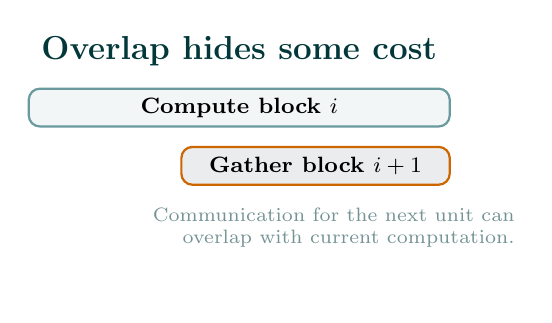
\begin{tikzpicture}[x=1cm,y=1cm]
  % bounding box height 3.373cm = table height, so the tealbox below starts
  % level with the bluebox; bars span the full column width, flush with the
  % heading, the tealbox and the takeaway
  \path (-2.673,0) rectangle (2.673,3.373);
  \node[font=\bfseries\large,text=mDarkTeal] at (0,3.09) {Overlap hides some cost};
  \draw[rounded corners=4pt,fill=tealBg,draw=tealBorder,thick] (-2.673,2.14) rectangle (2.673,2.62);
  \node[font=\footnotesize\bfseries] at (0,2.38) {Compute block $i$};
  \draw[rounded corners=4pt,fill=blueBg,draw=orange!80!black,thick] (-0.735,1.40) rectangle (2.673,1.88);
  \node[font=\footnotesize\bfseries] at (0.969,1.64) {Gather block $i+1$};
  \node[font=\scriptsize,text=mDarkTeal!55,align=right] at (1.2,0.85) {Communication for the next unit can\\overlap with current computation.};
\end{tikzpicture}}
\par\vspace{0.18cm}
\visible<4->{\begin{tealbox}{One-sentence summary}
\textbf{Shard most of the time; gather only when needed.}
\end{tealbox}}
\end{minipage}}
\par\vspace{0.22cm}
% the take node directly (not \takeaway) so no \begin{center} glue is added
\noindent\makebox[\linewidth]{\visible<5->{
\begin{tikzpicture}\node[take]{FSDP enables larger-model training by trading \textbf{memory} for \textbf{communication}.};\end{tikzpicture}}}
\end{frame}

\end{document}
